%RELATED

\subsection{Multiple Instance Learning}

The Multiple Instance Learning (MIL) problem was first described by Dietterich in the context of drug activity prediction \cite{dietterich97}. 
%In this problem, we want to figure out which of a number of different molecules will bind to a target ``binding site". 
Each molecule can assume a number of different 3-dimensional shapes (conformations), so even for molecules that are known to bind to the binding site, it is not necessarily known which conformation of the molecule succeeds in binding. If even one shape of a given molecule binds to a binding site, it is considered a ``good" molecule \cite{dietterich97}. Thus, in the original formation of MIL, a bag is classified as positive if one or more instances within it is positive, while a negative bag contains only negative instances. This is commonly referred to as the ``standard multiple instance assumption" \cite{amores13}. In the original paper, Dietterich developed a solution based on axis-parallel rectangles to solve this problem, and the MIL approach was shown to be significantly more effective than a standard supervised learning approach \cite{dietterich97}. In the late 1990s and early 2000s, a number of different approaches were developed for the original MIL problem, such as Diverse Density (DD) \cite{perez98}, EM-DD \cite{zhang01}, MI-SVM \cite{andrews02}, sbMIL \cite{bunescu07}, and MILES \cite{wang06}. A recent review of MIL by Amores created a taxonomy of these various methods and compared their effectiveness for classification \cite{amores13}. Most of these methods follow the standard assumption, which is not useful in real domains in which negative bags may contain some proportion of positive instances.
%

More recently, there has been increased interest in different formulations of the MIL problem. For instance, the problem of ``key instance detection" \cite{zhou12} revolves around finding the instances that contribute the most to bag labels. A recent study by Kotzias et al. focused on a formulation of the MIL problem in which bags with negative labels can contain some positive instances, and developed a general cost function for determining individual instance labels from group labels \cite{kotzias15}. This is significant in metagenomics because, while some diseases are caused by a single pathogen, many arise from a combination of many factors, and even patients that are healthy may contain small amounts of pathogens that are normally associated with disease. In contrast with the standard assumption, this can be referred to as the ``collective" assumption \cite{amores13}. Additionally, it is helpful to discover which microbes and which functional attributes of those microbes lead to disease, making instance level information significant in this domain.
%

While some of the above methods follow the standard assumption and others follow the collective assumption, they all treat bag labels simply as aggregations of instance labels and thus focus only on comparisons between individual instances and not entire bags or groups of instances. For methods following the standard assumption, the aggregation function is simply an OR function: if any of the instances in a bag are positive, the entire bag is positive. For methods following the collective assumption, the aggregation function is often based on an averaging of instance labels. Regardless of the problem assumption, methods that rely only on comparisons between individual instances are referred to as ``Instance Space" by Amores; this paradigm was generally  less effective than the two other paradigms, ``Bag Space" and ``Embedded Space" \cite{amores13}. Bag Space methods define a distance or kernel function that determine the similarity between bags, while Embedded Space methods map bags into feature vectors which can then be used for classifiers \cite{amores13}. Embedded Space methods can be further divided into two subcategories: methods that simply aggregate information about all instances in a bag without differentiating them, and ``Vocabulary-based" methods that group certain similar instances together and then use those groups to form the feature vector \cite{amores13}. We use a vocabulary-based method in this paper, because having information about groups of similar sequence reads can be biologically important, as explained further in the clustering section.

The Multiple Instance paradigm fits phenotype prediction well, since we have a set of labeled patients containing unlabeled sequence reads, and we would like to predict both the patient phenotype and which reads are indicative of that phenotype. Despite the recent developments in MIL and its potential utility in phenotype prediction, we have not found any literature that specifically applies MIL to classifying patient phenotype based on metagenomic data.

\subsection{Assembly}

%\begin{figure}[h]
%\centering
%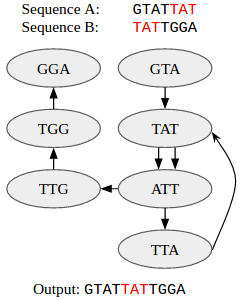
\includegraphics[scale=0.5]{./de-bruijn.png}
%\caption{This diagram illustrates a basic de Bruijn graph, as explained in the text. Notice the double arrow from TAT to ATT, allowing a path to go through that route twice. Thus, the longest contig that can be created by following a path is GTATTATTGGA, which is what we want.} \label{de-bruijn}
%\end{figure}

The \emph{assembly} problem involves combining overlapping short reads (usually less than 1000 base pairs) into longer sequences called \emph{contigs} (often tens of thousands of base pairs). For instance, if one read ends with the same relatively large nucleotide string that another read starts with, the reads are likely to be overlapping fragments from the same genome, and can thus be combined into one contig. This can be done either \emph{de novo} (in an unsupervised manner) or by referencing sequences against known contigs. We focus on de novo assembly, in order to keep our pipeline as unsupervised as possible. 

One of the main purposes of assembly is to determine the whole genomes of microbial species, the vast majority of which have not or cannot be laboratory cultured, from sequencing reads \cite{zerbino08}. Even if complete genomes cannot be assembled, combining reads into larger contigs can still make them much more useful for clustering and classification, because the contigs will contain more phylogenetic and functional information than short reads. This is because short reads of less than 1000 base pairs constitute only a tiny fraction of microbial genomes, which are usually hundreds of thousands to millions of base pairs, making it difficult to ascertain much about the phylogeny of individual reads. Many modern sequence reads are produced by Next-Generation and High-Throughput Sequencers, which usually produce these short reads. Metagenomics additionally poses its own set of challenges, due to very large datasets and lack of knowledge about how many species are present and in what relative abundances \cite{namiki12}. Thus, metagenome assembly is a relatively new and challenging field. Some popular single genome and metagenome assembly approaches include SOAPdenovo2 \cite{luo12}, IDBA-UD \cite{peng12}, Velvet \cite{zerbino08}, MetaVelvet \cite{namiki12}, ABySS \cite{simpson09}, and Ray Meta \cite{boisvert12}. Here we use SOAPdenovo2 because it was the assembler used by Qin et al. in their metagenomics study \cite{qin041012}.
%There are variations on how exactly de Bruijn graphs are represented and implemented, but Figure \ref{de-bruijn} illustrates the general process.

\subsection{Clustering}


%\begin{figure}[h]
%\centering
%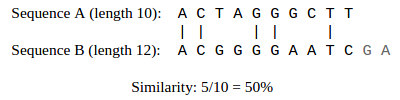
\includegraphics[scale=0.5]{./uclust-similarity.png}
%\caption{This diagram illustrates the similarity computation between two sequences in UCLUST. Terminal characters are excluded, so the length of the reads is 10. In the first 10 characters of each string, there are 5 matching characters that are in the same position in the string. Thus, the similarity is 5/10 = 50\%.} \label{uclust-similarity}
%\end{figure}

The \emph{clustering} problem in this context  involves grouping input short sequences (reads or contigs)   such that sequences 
within a group are similar to each other. The clusters 
obtained from this process are referred to 
as Operational Taxonomic Units (OTUs). OTUs represent a 
group of equivalent or similar organisms. Accordingly, the 
number of OTUs in a sample gives an approximation of the 
species diversity in that sample  \cite{schloss2009introducing,schloss2005introducing,sun2009esprit}.
In addition to approximating species diversity, clustering has several other key advantages. Because 
clustering is always de novo (unsupervised), it 
is not limited by the species that are 
covered in taxonomic databases. This is  important 
because it is believed that most micro-organisms that reside 
in the human body have not been laboratory cultured \cite{handelsman04}. Clustering also reduces computational 
costs by allowing analyses to operate on entire clusters instead of 
on each read/contig. Finally, clustering helps 
the classification process by allowing feature vectors to be built
at the OTU level, instead of using individual short reads. UCLUST \cite{Edgar10}, CD-HIT \cite{Li01072006}, mothur \cite{schloss2009introducing}, DOTUR \cite{schloss2005introducing}, CROP \cite{Hao01032011}, and MC-MinH \cite{sdm2013a} are some of the popular sequence clustering approaches. 

% Not needed for a bioinf. audience
%This is illustrated in figure \ref{uclust-similarity}.
